\chapter{WYNIKI TESTÓW}
\label{chapter:wyniki_testow}

\section{API Wit.ai}
\label{section:witai}
W celu przetestowania działania modelu językowego opracowanego na platformie Wit.ai przeprowadzono testy na przykładowych zdaniach. Do testów przygotowano zdania, które użytkownik aplikacji mógłby zadać. Poniżej przedstawiono pytania wykorzystane pdczas testów:

\begin{itemize}
    \item Add bread from biedronka to cart
    \item Add bread to cart
    \item Go to cart
    \item What is this?
\end{itemize}


W celu przetestowania przepływu interaktywnego, w którym system oczekuje od użytkownika odpowiedzi, w celu zrealizowania akcji, wykorzystano zapytanie \textit{Add bread from biedronka to cart}. System prawidłowo rozpoznał encję \textit{product} oraz \textit{store}. System pyta użytkownika, czy dodany ma zostać tylko jeden bochenek chleba. Po otrzymaniu pozytywnej odpowiedzi, system zwraca do aplikacji informację, że należy dodać dany produkt do koszyka. W przypadku gdyby któraś z encji nie zostałą rozpoznana, system zadałby pytanie z prośbą o uzupełnienie kontekstu. Przykład takiego zachowania przedstawiono na rysunku \ref{fig:witai_context_example}.
\begin{figure}[H]
    \centering
    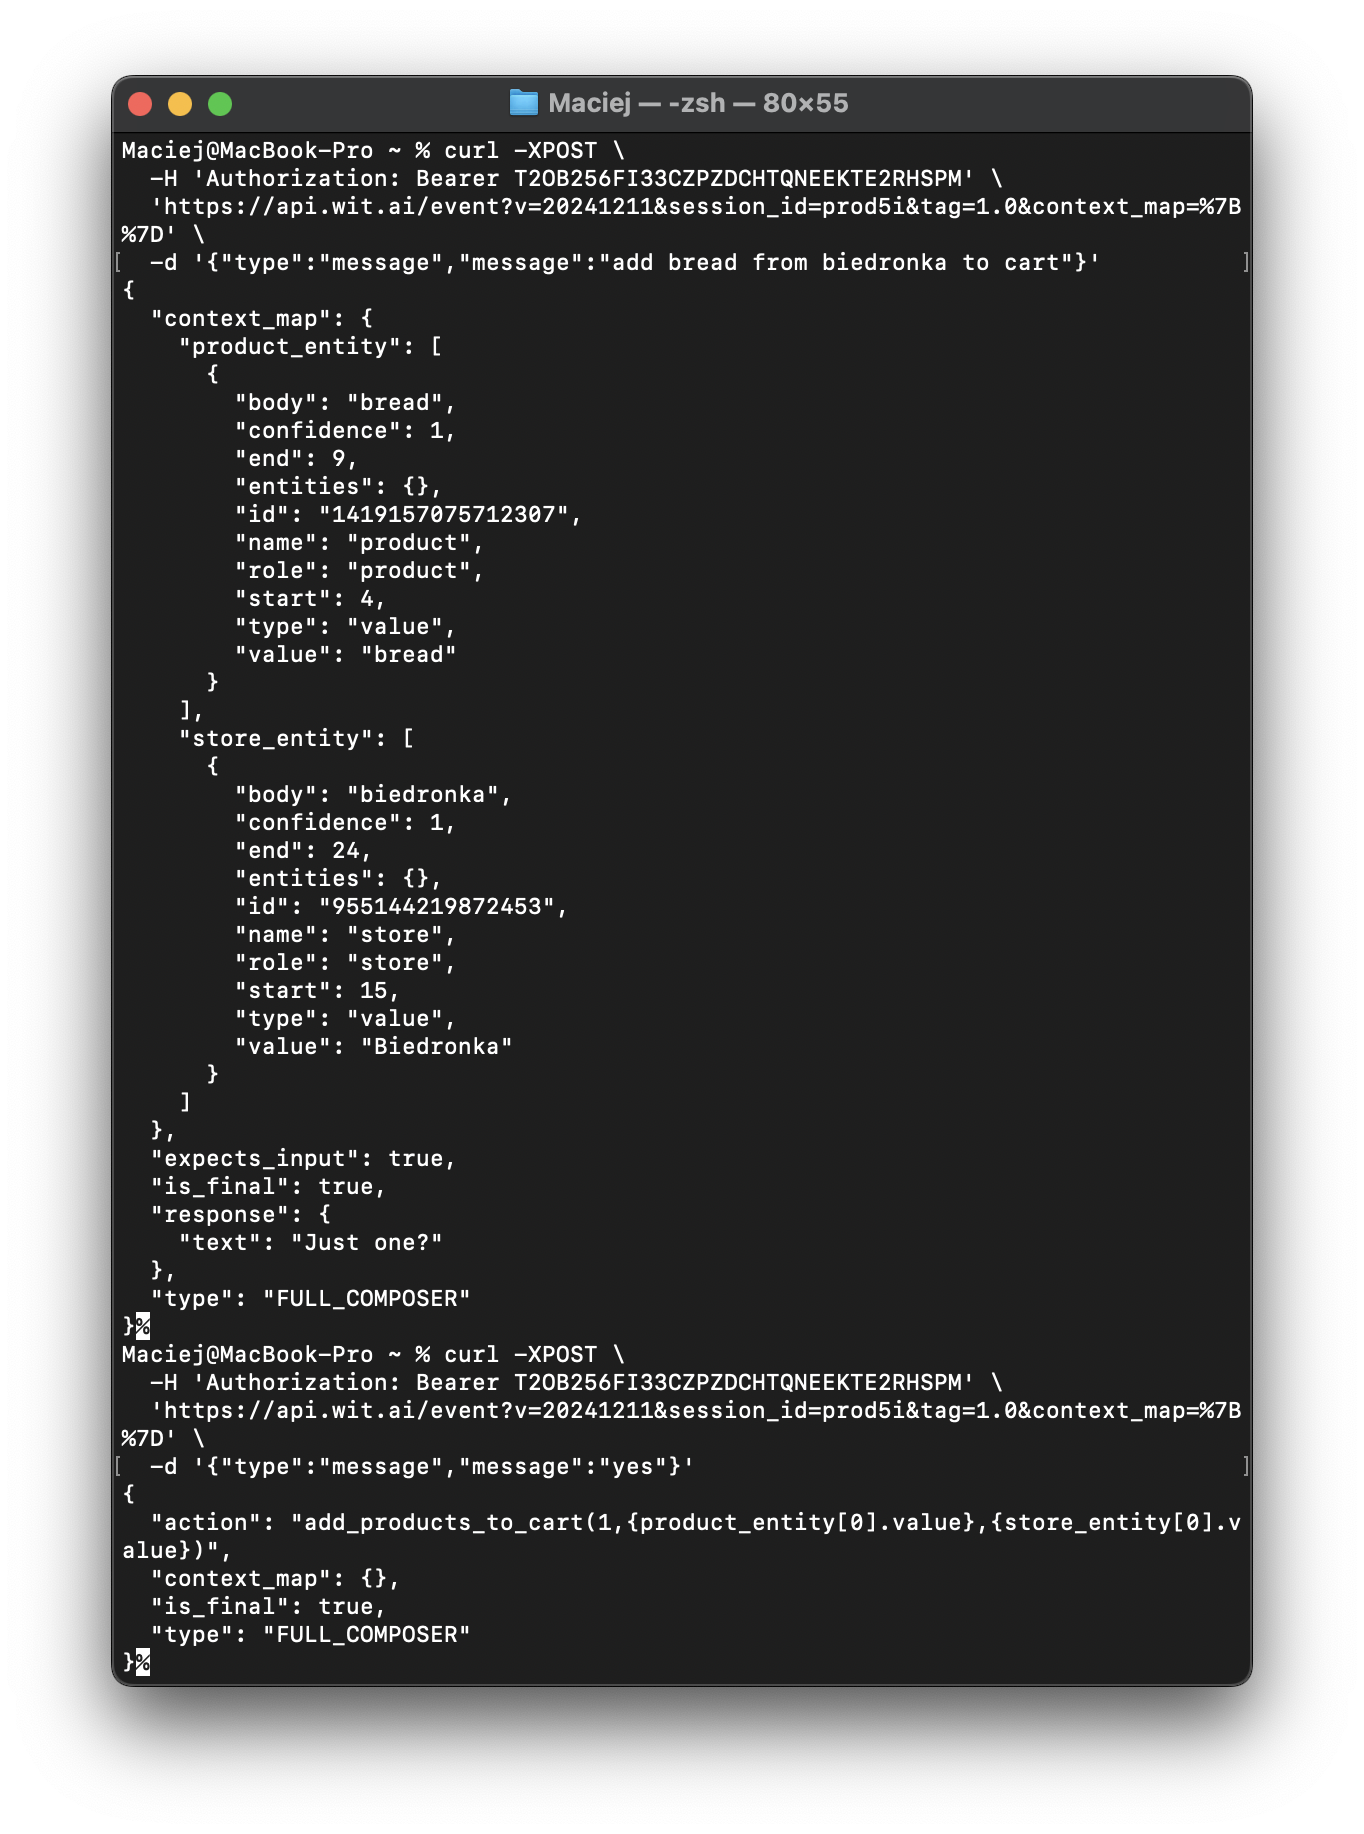
\includegraphics[width=0.8\textwidth]{images/witai_complex_convo.png}
    \caption{Przykład kompleksowej konwersacji z systemem Wit.ai}
    \label{fig:witai_complex_convo}
\end{figure}

\begin{figure}[H]
    \centering
    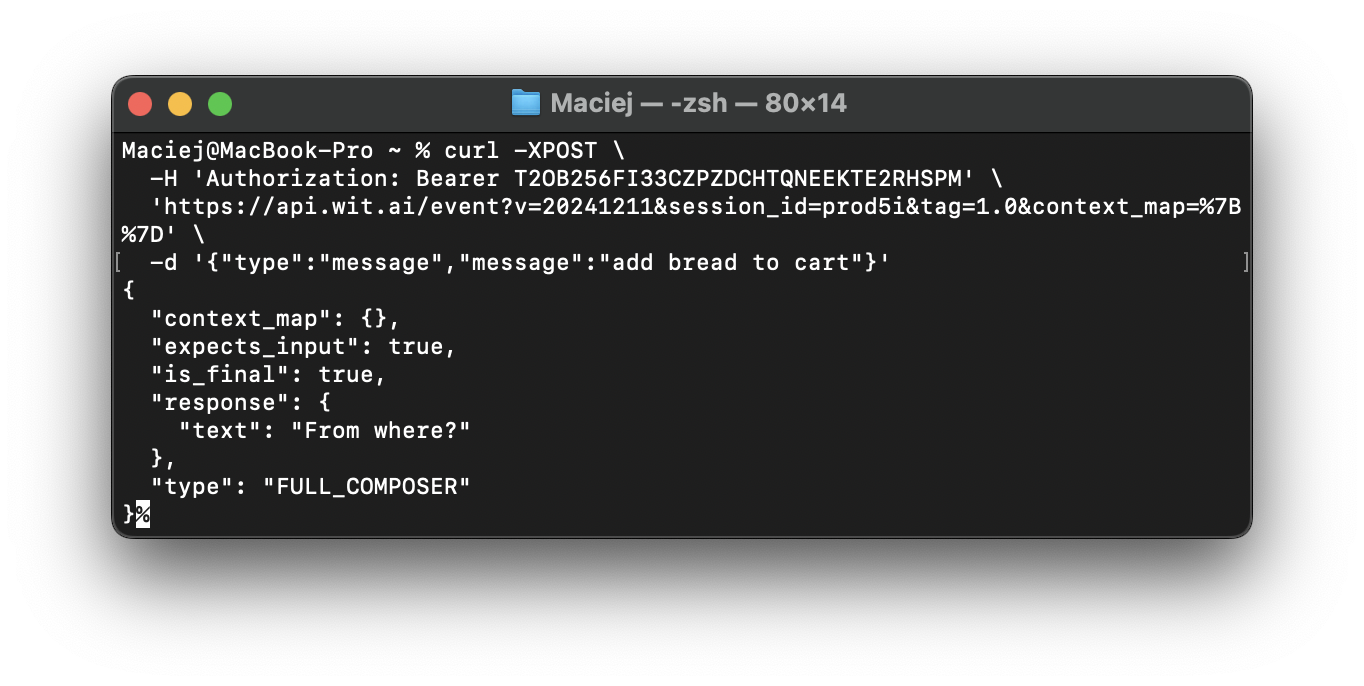
\includegraphics[width=0.8\textwidth]{images/witai_context_example.png}
    \caption{Przykład pytania systemu Wit.ai o uzupełnienie kontekstu}
    \label{fig:witai_context_example}
\end{figure}

Jak widać na rysunku \ref{fig:witai_context_example}, system zapytał użytkownika o uzupełnienie kontekstu, gdyż nie otrzymał informacji na temat sklepu.

\begin{figure}[H]
    \centering
    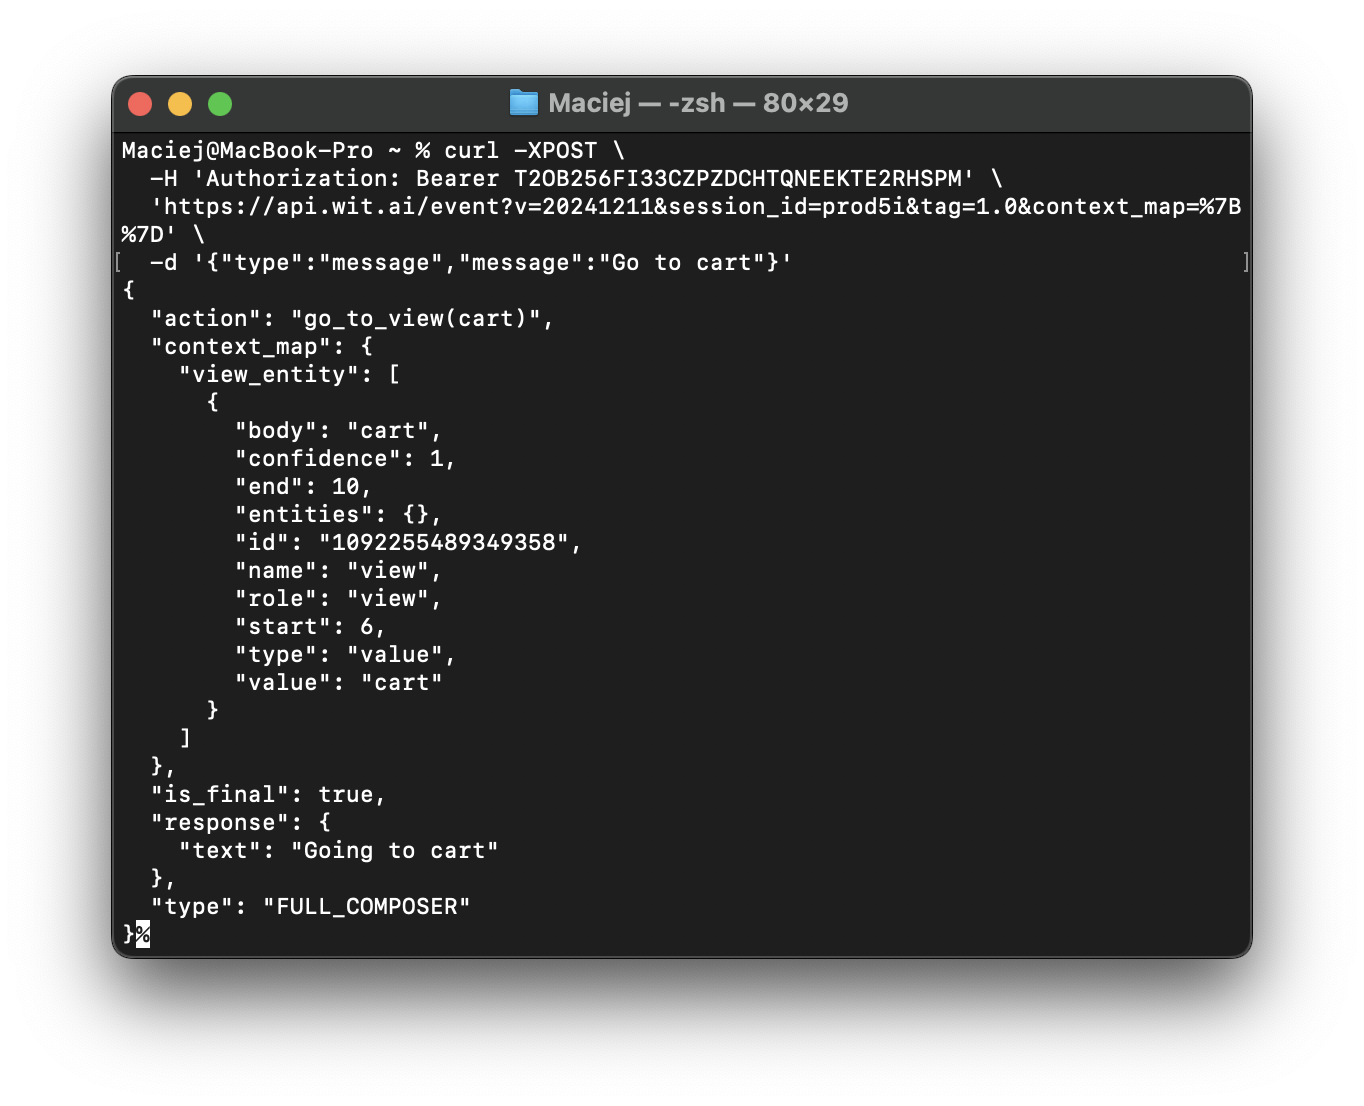
\includegraphics[width=0.8\textwidth]{images/witai_go_to_cart.png}
    \caption{Przykład przejścia do widoku koszyka}
    \label{fig:witai_cart_example}
\end{figure}

Na rysunku \ref{fig:witai_cart_example} przedstawiono przykład przejścia do widoku koszyka. System poprawnie zrozumiał zapytanie i zwrócił odpowiedź, że użytkownik chce przejść do koszyka.

\begin{figure}
    \centering
    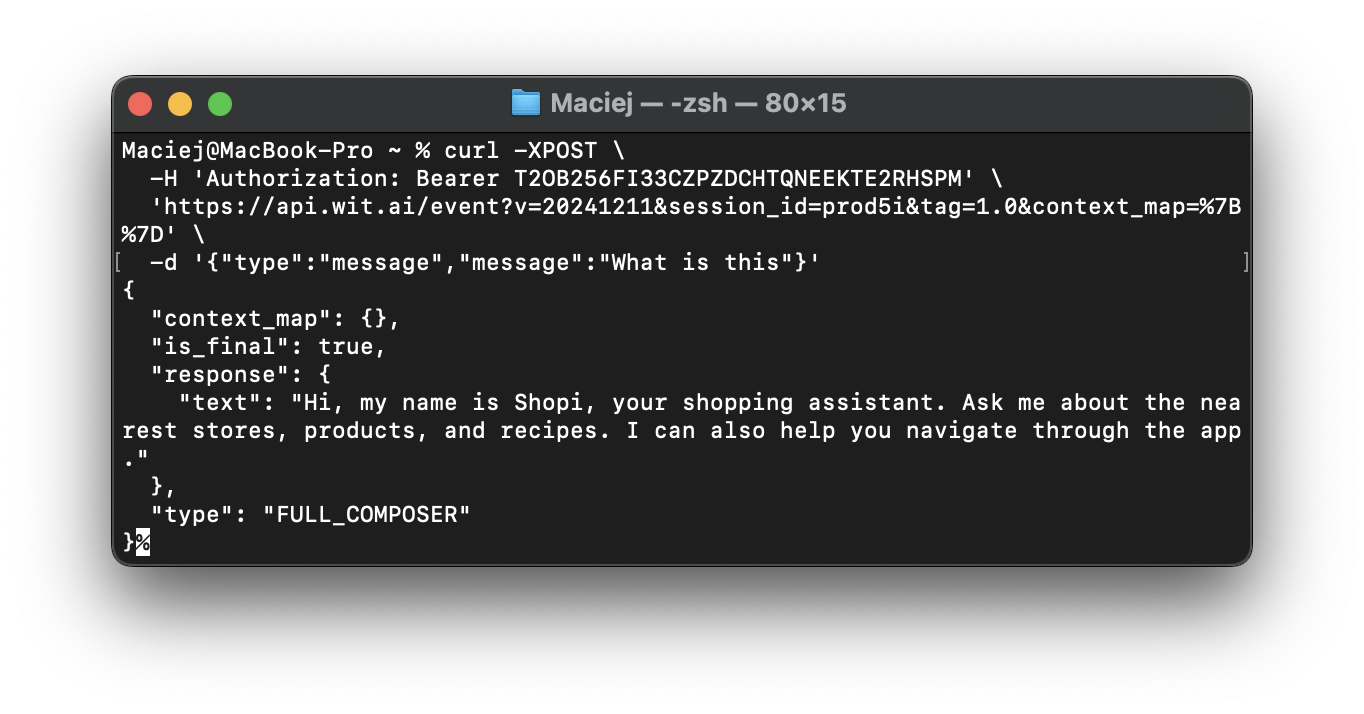
\includegraphics[width=0.8\textwidth]{images/witai_what_is_this.png}
    \caption{Przykład zapytania o nazwę produktu}
    \label{fig:witai_what_is_this}
\end{figure}

Na rysunku \ref{fig:witai_what_is_this} przedstawiono przykład zapytania zakłopotanego użytkownika, który nie wie, co to jest. System w odpowiedzi na takie pytanie, przedstawił się, co jest oczekiwanym zachowaniem.